% Moiré is counting -- the theory paper. Build: tectonic -X compile paper2.tex --outdir build
%
% This is the shell; the sections are p2-*.tex, every quoted number is a macro
% in numbers.tex (generated by tools/numbers.mjs, which refuses to build over a
% failing experiment gate), and the predictions table is tab-predictions.tex,
% generated the same way. The class is provisional: the venue is decided with
% the finished draft in hand (paper/notes/paper2-plan.md, P5).
\documentclass[10pt]{article}
\usepackage[margin=1.05in]{geometry}
\usepackage{amsmath}
\usepackage{amssymb}
\usepackage{amsthm}
\usepackage{booktabs}
\usepackage{graphicx}
\usepackage{xcolor}
\usepackage{microtype}
\usepackage{tikz}
\usepackage{pgfplots}
\pgfplotsset{compat=1.18}
\usetikzlibrary{arrows.meta}
\usepackage[colorlinks=true, linkcolor=cool, citecolor=cool, urlcolor=cool]{hyperref}
\graphicspath{{figures/}}

\definecolor{ink}{HTML}{15181C}
\definecolor{accent}{HTML}{C81E5A}
\definecolor{cool}{HTML}{1B6CA8}
\definecolor{warm}{HTML}{D4761A}
\definecolor{soft}{HTML}{8A94A0}

\theoremstyle{plain}
\newtheorem{theorem}{Theorem}[section]
\newtheorem{proposition}[theorem]{Proposition}
\newtheorem{lemma}[theorem]{Lemma}
\newtheorem{corollary}[theorem]{Corollary}
\theoremstyle{definition}
\newtheorem{definition}[theorem]{Definition}
\newtheorem{remark}[theorem]{Remark}

\newcommand{\R}{\mathbb{R}}
\newcommand{\Z}{\mathbb{Z}}
\newcommand{\tor}{\mathbb{T}}
\newcommand{\E}{\mathbb{E}}
\newcommand{\Rot}[1]{\mathbf{R}_{#1}}
\newcommand{\rad}{\rho}
\newcommand{\idx}{\phi}
\newcommand{\het}{\eta}
\newcommand{\Moire}{\textsc{Moir\'e}}
\newcommand{\figlead}[1]{\textbf{#1}\ }
% A figure that does not exist yet: what it will show, and which script owns it.
\newcommand{\placeholder}[2]{%
  \begin{center}\fbox{\parbox{0.92\linewidth}{\centering\vspace{1.6em}%
    \textbf{Figure: #1}\\[0.4em]\small #2\vspace{1.6em}}}\end{center}}

% GENERATED by paper/tools/numbers.mjs -- do not edit by hand.
% Every number the prose quotes, in one place, so text and data cannot drift.

% ---- src/types/moire.ts : what the Studio offers
\newcommand{\fieldCount}{six}
\newcommand{\patternCount}{thirteen}
\newcommand{\envTaps}{24}

% ---- data/fringe.json : the fringe law
\newcommand{\fringeScenes}{12}
\newcommand{\fringeSamples}{107{,}691}
\newcommand{\fringeMeanErr}{0.0034}
\newcommand{\fringeWorstP}{0.073}
\newcommand{\fringeLight}{0.036}
\newcommand{\fringeDark}{0.416}
\newcommand{\fringeRegime}{1/4}

% ---- data/lawatlas.json : admitted fraction per panel
\newcommand{\atlasCombs}{100.0}
\newcommand{\atlasCircleLines}{39.1}
\newcommand{\atlasHex}{93.5}
\newcommand{\atlasCircles}{21.7}
\newcommand{\atlasControl}{0.0}

% ---- data/gradient.json : the missing gradient divide
\newcommand{\gradWorstWave}{25.2}
\newcommand{\gradWorstHyp}{14.8}
\newcommand{\gradWorstSpiral}{7.3}
\newcommand{\gradWorstParab}{224}
\newcommand{\gradWaveFrame}{61}
\newcommand{\gradHypFrame}{66}
\newcommand{\gradParabFrame}{98}
\newcommand{\gradSpiralFrame}{0}

% ---- data/gpu.json : 1200x800 = 0.96 Mpixel, one full-screen layer
\newcommand{\gpuSpeedLo}{11}
\newcommand{\gpuSpeedHi}{37}
\newcommand{\gpuTriRotOne}{14.4}
\newcommand{\gpuTriRotOneNew}{0.39}
\newcommand{\gpuTriRotOffOut}{27.9}
\newcommand{\gpuTriRotOffOutNew}{1.64}
\newcommand{\gpuSquareOld}{0.92}
\newcommand{\gpuSquareClosed}{0.20}
\newcommand{\gpuSquareClosedGain}{4.7}
\newcommand{\gpuAdapter}{metal-3}

% ---- data/gpu.json : interpreting a field expression against unrolling it
\newcommand{\interpPerOp}{0.103}
\newcommand{\interpLo}{0.63}
\newcommand{\interpHi}{6.9}
\newcommand{\interpHiOps}{67}
\newcommand{\unrolledLo}{0.0043}
\newcommand{\unrolledCeil}{0.054}
\newcommand{\fieldBaseline}{0.0071}
\newcommand{\fieldEmptyCost}{0.044}
\newcommand{\fieldEmptyGain}{6}
\newcommand{\fieldOpsLo}{6}
\newcommand{\fieldOpsHi}{67}
\newcommand{\fieldStmtHi}{73}
\newcommand{\fieldTwinWorst}{4{\times}10^{-5}}
\newcommand{\fieldGainLo}{40}
\newcommand{\fieldGainHi}{265}

% ---- data/cost.json : CPU metric evaluations per pixel, mean
\newcommand{\costScenes}{7}
\newcommand{\costSweepLo}{180}
\newcommand{\costSweepHi}{361}
\newcommand{\costOursLo}{7.5}
\newcommand{\costOursHi}{11.1}
\newcommand{\costVsSweepLo}{18}
\newcommand{\costVsSweepHi}{33}
\newcommand{\costVsRefLo}{1.7}
\newcommand{\costVsRefHi}{9.4}

% ---- data/artifacts.json
\newcommand{\artHolesSweepDiff}{8.6}
\newcommand{\artHolesSweepEv}{1100}
\newcommand{\artHolesOursEv}{72}
\newcommand{\artHolesSaving}{15}
\newcommand{\artDriftLooseDiff}{38.3}
\newcommand{\artDriftRefInk}{0.459}
\newcommand{\artDriftLooseInk}{0.152}
\newcommand{\artAnchorEv}{33}
\newcommand{\artAnchorRefInk}{0.489}
\newcommand{\artAnchorLatticeInk}{0.216}
\newcommand{\artAnchorPixelInk}{0.216}

% ---- data/fidelity.json : the sweep against the exhaustive reference
\newcommand{\fidSettings}{2{,}401}
\newcommand{\fidLegible}{1{,}534}
\newcommand{\fidSweepHoles}{160}
\newcommand{\fidSweepWorst}{32.9}
\newcommand{\fidSweepLegibleHoles}{3}
\newcommand{\fidSweepLegibleWorst}{4.2}
\newcommand{\fidSweepEnvelopeHoles}{41}
\newcommand{\fidSweepEnvelopeWorst}{29.6}
\newcommand{\fidLooseHoles}{46}
\newcommand{\fidLooseWorst}{48.3}
\newcommand{\fidLooseEnvelopeHoles}{13}
\newcommand{\fidOursHoles}{146}
\newcommand{\fidOursWorst}{13.8}

% ---- data/saturation.json : the interval-width sweep
\newcommand{\satSettings}{55{,}692}
\newcommand{\satFitting}{45{,}774}
\newcommand{\satFittingPct}{82}
\newcommand{\satStrided}{9{,}918}
\newcommand{\satWidestFitting}{1022}
\newcommand{\satMedianInk}{0.89}
\newcommand{\satStridedLegible}{1{,}472}
\newcommand{\satStridedLegiblePct}{2.6}
\newcommand{\satBudget}{1{,}024}
\newcommand{\satDriftRatioHi}{4.2}

% ---- data/degenerate.json : strided band against a deep scan
\newcommand{\degChecked}{534}
\newcommand{\degWithDrop}{217}
\newcommand{\degWorst}{48.8}
\newcommand{\degMean}{4.6}
\newcommand{\degLegible}{298}
\newcommand{\degLegibleWorst}{28.7}

% ---- data/residual.json : the worked pixel of the window figure
\newcommand{\figNaive}{49}
\newcommand{\figTrue}{41}
\newcommand{\figGap}{8}
\newcommand{\figLo}{22}
\newcommand{\figHi}{56}
\newcommand{\figSpan}{35}
\newcommand{\figEvals}{9}
\newcommand{\figGuard}{10.5}
\newcommand{\figSpacing}{14}

% ---- data/window.json : the interval checked against a brute-force argmin
\newcommand{\winChecks}{13{,}458}
\newcommand{\winViolations}{0}

% ---- data/ablation.json : one mechanism removed, time relative to full
\newcommand{\ablSkipLo}{2.1}
\newcommand{\ablSkipHi}{3.3}
\newcommand{\ablClosedMarginal}{90.3}
\newcommand{\ablCostLo}{8}
\newcommand{\ablCostHi}{19}
\newcommand{\ablMpixel}{3.84}

% ---- data/zoom.json : zoom stability
\newcommand{\zoomDecades}{1.2}
\newcommand{\zoomRefSamples}{36}
\newcommand{\zoomCoarsestPeriod}{1.5}
\newcommand{\zoomFloorNoise}{0.046}
\newcommand{\zoomNoFloorNoise}{0.115}
\newcommand{\zoomValueNoise}{0.118}
\newcommand{\zoomFloorNoiseCoarse}{0.002}
\newcommand{\zoomNoFloorNoiseCoarse}{0.115}
\newcommand{\zoomNoiseRatio}{77}
\newcommand{\zoomFloorInkGain}{0.61}
\newcommand{\zoomValueBias}{0.004}

% ---- data/contour.json : moire as a contouring primitive
\newcommand{\contourCarrier}{5}
\newcommand{\contourDetune}{5.5556}
\newcommand{\contourCtlGap}{50}
\newcommand{\contourFloor}{0.22}
\newcommand{\contourFloorP}{0.61}
\newcommand{\contourBestErr}{0.23}
\newcommand{\contourWorstErr}{0.58}
\newcommand{\contourAtFloor}{three}
\newcommand{\contourAtFloorErr}{0.25}
\newcommand{\contourFieldCount}{six}
\newcommand{\contourWorstP}{2.62}
\newcommand{\contourProbes}{63{,}904}
\newcommand{\contourFinest}{8.14}
\newcommand{\contourDipoleResolved}{86}
\newcommand{\contourDipoleFinest}{8.14}


\title{Moir\'e is counting\\[0.3em]\large A theory of beats without frequencies}
\author{}
\date{Skeleton, \today}

\begin{document}
\maketitle

\begin{abstract}
A pattern is a counting map $\Phi$ into a torus, composed with an ink potential.
Everything visible about interference is one of three finite questions about
$\Phi$: which integer characters are slow (arithmetic), which survive an average
(analysis), and how the count fails to be a function (topology). Fourier appears
only as amplitude bookkeeping, and its one job, harmonic weights, is what prices
the arithmetic. Every claim below is measured by a script in the repository, and
the numbers are generated, never typed.
\end{abstract}

\section{The object}
\label{sec:object}

% P4: write this section last, once the laws exist. Related work lives here in
% one column: the indicial method as the (1,-1) germ (Amidror's own verdict,
% "ignores intensity profiles", names what the amplitude weight restores);
% Fourier theory global and periodic; de Bruijn's index function as a counting
% map asked different questions; the hull torus of incommensurate physics, the
% same torus asked spectral questions.

\begin{definition}[Counting map, ink potential, drawing]
\label{def:drawing}
A stack of $K$ scalar-index layers is a map
\[
  \Phi:\R^2\to\tor^K,\qquad \Phi(p)=\big(\idx_1(p),\dots,\idx_K(p)\big)\bmod 1,
\]
whose $i$-th coordinate is the fractional member index of layer $i$ at $p$,
together with an ink potential $I:\tor^K\to[0,1]$, the paint-order composite
of the per-coordinate stroke profiles. The drawing is $D=I\circ\Phi$.
\end{definition}

\begin{definition}[Characters, local frequency, slowness]
\label{def:character}
A character is $k\in\Z^K=H^1(\tor^K;\Z)$, acting as $\chi_k(x)=e^{2\pi i\,k\cdot x}$.
Its pullback $k\cdot\Phi$ has local frequency $J_p^{\top}k=\nabla(k\cdot\Phi)(p)$
with $J_p=D\Phi(p)$, and $k$ is \emph{slow} at $p$ when $|J_p^{\top}k|$ is small
against the carriers $|J_p^{\top}e_i|$. A moir\'e is the pullback of a slow
character.
\end{definition}

\begin{remark}[Fourier is bookkeeping]
For a product potential $I=\prod_i g_i(x_i)$, $\hat I(k)=\prod_i\hat g_i(k_i)$,
and a stroke's harmonics decay like $|\hat g(n)|\sim 1/n$. The amplitude weight
$|k_1k_2\cdots|$ of \S\ref{sec:selection} is this decay and nothing else; no
other Fourier statement is used.
\end{remark}

\placeholder{a stack beside its torus}{A two-layer stack and $\tor^2$: the
carriers as the fast directions of $D\Phi$, one slow character as a line on
the torus, the sweep's orbit as a closed geodesic. The only diagram in the
paper that is not a render. (P3.)}

\section{Law I: selection, the arithmetic of the visible beat}
\label{sec:selection}

\begin{definition}[Weighted merit]
\label{def:merit}
For a pair with index gradients $g_1,g_2$ and a character $(a,b)$ with $ab\ne0$,
\[
  \het_{a,b}\;=\;\frac{|a g_1+b g_2|}{\tfrac12\,|a g_1-b g_2|}\;\cdot\;|ab|,
\]
the heterodyne ratio of the beat against the carriers that form it, priced by
the harmonics that carry it. The visible character is the minimiser;
$\het<\tfrac14$ is the fringe regime.
\end{definition}

\begin{proposition}[Selection is reduction]
\label{prop:selection}
The minimiser of $\het_{a,b}$ over $\Z^2\setminus\{ab=0\}$ lies in the window
$\{i\,s+j\,t : |i|\le3,\ j\in\{1,2\}\}$ of a Lagrange--Gauss reduced basis
$(s,t)$ of the gradient lattice $\{a g_1+b g_2\}$. For parallel carriers of
pitch ratio $x$ the record-setting characters are the continued-fraction
convergents of $x$ (\selRecordsMatch\ records over \selRatios\ ratios, all
convergents); an order cap $|a|,|b|\le2$ misses \selCapMissPct\% of the
visible fringes of random pairs, the window misses \selShipMiss.
\end{proposition}

\begin{figure}[t]
  \centering
  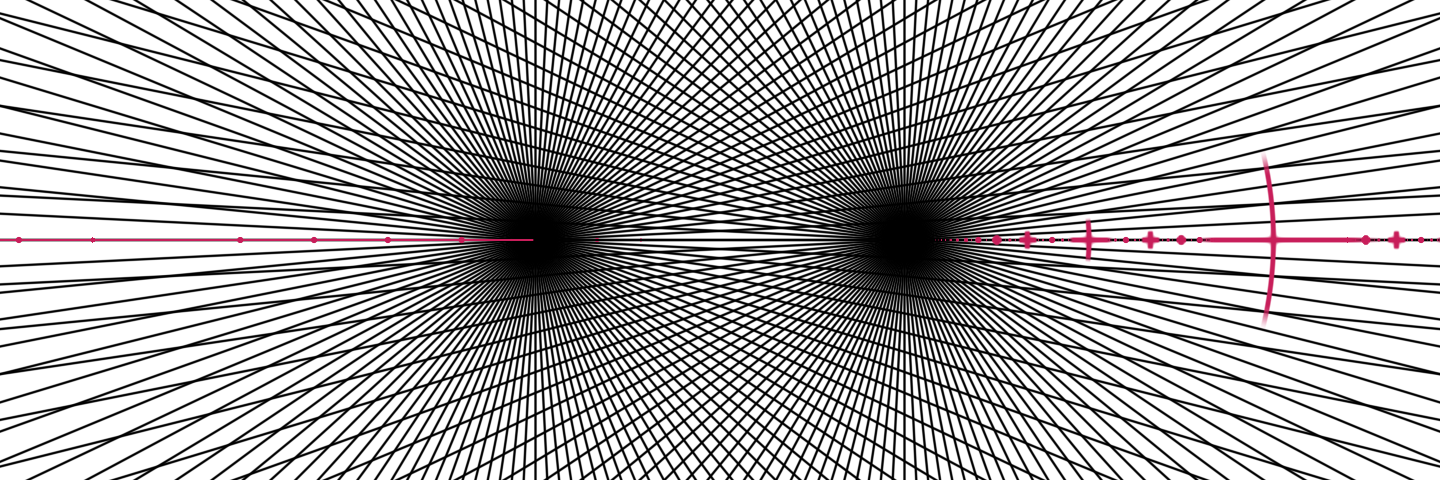
\includegraphics[width=\linewidth]{selection-stations.png}
  \caption{\figlead{Stations as places.} Two radial fans off-centre: along
  the axis between them the local pitch ratio sweeps the rationals, and each
  rational the amplitude weight admits owns a commensurate pocket, whose
  winning character's level sets are drawn in accent — the convergent ladder
  as geography. Provisional: the companion's stations strip
  (\texttt{selectionfigs.mjs}); the weighted staircase joins it at P4.}
  \label{fig:stations}
\end{figure}

\begin{theorem}[Duty nulls]
\label{thm:dutynull}
The visible station of a $p{:}q$ pair (coarse\,:\,fine) is the character
$(q,-p)$, carried by the coarse family's $q$-th profile harmonic and the fine
family's $p$-th. A stroke of duty $d$ has vanishing $q$-th harmonic exactly when
$qd\in\Z$, so the station is extinguished at rational coarse duties and
nowhere else. Measured on the station over strips holding a whole number of
every period: the $2{:}1$ null at $d=\tfrac12$ is $\dutyNullDepthTwo\times$ below
its neighbours, the $3{:}1$ nulls at $\tfrac13$ and $\tfrac23$ are
$\dutyNullDepthThreeLow\times$ and $\dutyNullDepthThreeHigh\times$, and away from
the nulls the amplitudes track $|\sin(q\pi d)/q\pi|$ within \dutyNullLawPct\%,
the anti-alias ramp's softening.
\end{theorem}

\begin{figure}[t]
  \centering
  \begin{minipage}[c]{0.4\linewidth}
    \centering
    \begin{tikzpicture}
      \begin{axis}[width=\linewidth, height=4.9cm, xlabel={coarse duty $d$},
        ylabel={$|\hat I(q,-1)|$}, xmin=0.18, xmax=0.82, ymin=0, ymax=0.045,
        scaled y ticks=false, ytick={0,0.01,0.02,0.03,0.04},
        tick align=outside, tick pos=left, axis line style={gray!60},
        grid=major, grid style={gray!18, very thin},
        label style={font=\footnotesize}, tick label style={font=\scriptsize},
        legend style={font=\scriptsize, draw=gray!40, at={(0.5,1.02)}, anchor=south, legend columns=2},
        xtick={0.25,0.333,0.5,0.667,0.75}, xticklabels={$\frac14$,$\frac13$,$\frac12$,$\frac23$,$\frac34$}]
        \addplot[accent, line width=0.7pt] table[x=duty, y=two, col sep=comma]{data/dutynull-law.csv};
        \addlegendentry{$2{:}1$, $(2,-1)$}
        \addplot[cool, line width=0.7pt] table[x=duty, y=three, col sep=comma]{data/dutynull-law.csv};
        \addlegendentry{$3{:}1$, $(3,-1)$}
        \addplot[accent, only marks, mark=*, mark size=1.3pt] table[x=duty, y=two, col sep=comma]{data/dutynull-curve.csv};
        \addplot[cool, only marks, mark=square*, mark size=1.1pt] table[x=duty, y=three, col sep=comma]{data/dutynull-curve.csv};
      \end{axis}
    \end{tikzpicture}
  \end{minipage}\hfill
  \begin{minipage}[c]{0.57\linewidth}
    
\includegraphics[width=\linewidth]{dutynull-triple.png}
  \end{minipage}
  \caption{\figlead{Duty nulls.} Left: the station's amplitude against the
  coarse stroke's duty, measured on the shipped compositing (marks) over the
  hard-ink law $|\sin(q\pi d)/q\pi|\,|\hat g_{\text{fine}}(1)|$ (lines): the
  $2{:}1$ station dies at $d=\tfrac12$, the $3{:}1$ station at $\tfrac13$
  and $\tfrac23$, and the soft stroke's ramp is the only departure. Right:
  the $2{:}1$ pair's station envelope, the exposure at rates $(1,2)$ of
  Theorem~\ref{thm:exposure} expanded sixfold about its mean, at coarse duty
  $0.35$, $0.5$ and $0.65$: present, extinguished, present. Scripts
  \texttt{dutynull.mjs}, \texttt{dutynull-figs.mjs}.}
  \label{fig:dutynull}
\end{figure}

\begin{definition}[Visibility spectrum of a real number]
\label{def:visibility}
For $x>0$, the visibility spectrum is the staircase
$\nu_x(N)=\min\{\,|p-qx|\cdot pq:\ p,q\ge1,\ pq\le N\,\}$: best approximation
with denominators priced by the product $pq$ rather than by $q$. Its record
holders are the visible stations of a $1{:}x$ pair. We know of no name for this
object in the number-theoretic literature.
\end{definition}

\section{Law II: averaging, the envelope as a conditional expectation}
\label{sec:averaging}

\begin{theorem}[The envelope is a conditional expectation, and a sharp one]
\label{thm:envelope}
For a schedule $w\in\Z^K$ let $\mathcal E_w I(x)=\int_0^1 I(x+uw)\,du$. Then
\[
  \widehat{\mathcal E_w I}(k)\;=\;\hat I(k)\cdot\mathbf 1[k\cdot w=0],
  \qquad\text{i.e.}\qquad
  \mathcal E_w I \;=\; \E\big[\,I\,\big|\,L_w\,\big],\quad L_w=\{k:k\cdot w=0\}:
\]
one period of an integer schedule projects exactly onto the characters
annihilated by $w$, with no leakage.
\end{theorem}

\begin{corollary}[Four cases]
\label{cor:cases}
\emph{(i) Fringe law.} Two layers on the diagonal $w=(1,1)$: $\E[I\mid\idx_1-\idx_2]$
is a function of $D=\idx_1-\idx_2$ alone, the saturating tent.
\emph{(ii) Pivot.} $w$ incommensurate in every coordinate: $\E[I]$, the
independent-phase mean, the DC about which contrast is expanded.
\emph{(iii) Zero sums.} The diagonal $w=(1,\dots,1)$ preserves the whole
zero-sum lattice at once: every pairwise difference and every zero-sum ternary.
\emph{(iv) Exposure.} A stack animated at rates $r$ and averaged over one period
is $\mathcal E_r I$: a long exposure is an envelope.
\end{corollary}

\begin{theorem}[Exactness]
\label{thm:exact}
For an all-scalar stack every swept profile $\alpha_i(u)$ is piecewise cubic in
$u$ with corners known in closed form from the phase trio (the nearest member's
window and ramps, the floor clips, the argmin midpoints where a stroke reaches
them, the wrap seam), so $\mathcal E_w I(\Phi(p))$ is piecewise polynomial with
known breakpoints and is integrated in closed form. Certified on \exactScenes\
scenes across twelve regimes against a \exactTruthTaps-tap double-precision
truth: the shipped Gauss-3 chain is within $\exactWorstErr$ (one part in
\exactWorstGrayFrac\ of a gray level), a Gauss-4 pass within
$\exactGaussFourErr$, and the shipped shader within $\exactGpuErr$ of its
double-precision twin; \envTaps\ taps err by \exactTapsWorst\ of the tonal
range at the rate-12 station, and the chain beats them $\exactOverTaps\times$
at worst.
\end{theorem}

\begin{theorem}[Temporal selection]
\label{thm:exposure}
Averaging a stack animated at rates $r\in\Z^K$ over one period keeps exactly
the characters with $k\cdot r=0$. On the $16.4{:}8$ pair's station $(2,-1)$:
rates $(1,2)$ keep it to \exposureFaithfulPct\% of the still, while $(1,1)$ and
$(2,1)$ wash it $\exposureSelectivity\times$.
\end{theorem}

\begin{figure}[t]
  \centering
  
\includegraphics[width=\linewidth]{exposure-quad.png}
  \caption{\figlead{The shutter is a character filter.} The $16.4{:}8$ pair
  as a still, then its long exposures over one period at rates $(1,1)$,
  $(1,2)$ and $(2,1)$, each expanded sixfold about its own mean. The still's
  station is a four-percent modulation the page cannot show. Rates $(1,1)$
  keep the zero-sum characters — here the carrier-scale coefficient $(1,-1)$,
  a fine texture, not a fringe — and wash the station; rates $(1,2)$ keep
  exactly the station $(2,-1)$, the broad bands; rates $(2,1)$ wash both and
  keep the faster $(1,-2)$. Scripts \texttt{exposure.mjs},
  \texttt{exposure-figs.mjs}.}
  \label{fig:exposure}
\end{figure}

\subsection{The observer theorem}
\label{sec:observer}

\begin{proposition}[The envelope is the universal invariant of rephasing]
\label{prop:invariant}
For a closed subgroup $H\le\tor^K$ let $\E_H I=\int_H I(\cdot+h)\,dh$. Every
continuous linear functional $F$ on ink potentials that is invariant under
translation by $H$ satisfies $F=F\circ\E_H$, and every $G\circ\E_H$ is
invariant: the $H$-invariant linear observables are exactly the linear
observables of the envelope.
\end{proposition}

\begin{theorem}[A window is a multiplier on the torus]
\label{thm:multiplier}
Let $W\ge0$ be an even window with $\int W=1$ and second moment $m_2$, and
$W_\rho$ its dilate to scale $\rho$. For $\Phi\in C^2$ and
$\sum_k|k||\hat I(k)|<\infty$,
\[
  (D*W_\rho)(p)\;=\;\sum_{k\in\Z^K}\hat I(k)\,\widehat W\!\big(\rho\,J_p^{\top}k\big)\,
  e^{2\pi i\,k\cdot\Phi(p)}\;+\;R_\rho(p),
  \qquad
  |R_\rho(p)|\;\le\;\pi\,\lVert D^2\Phi\rVert\,m_2\,\rho^2\sum_k|k||\hat I(k)|,
\]
and to first order $R_\rho$ is the multiplier's own second derivative in
frequency. Verified: exact to $\obsMultiplierErr$ without curvature; with it,
the second-derivative term leaves $\obsRemainderResidual$ of the remainder.
\end{theorem}

\begin{theorem}[Universality of the third pattern]
\label{thm:universality}
Every observer that pools before it decides, $O=A_\rho\circ N$ with $N$
pointwise and $A_\rho$ a window, reports at $p$ the potential $N\circ I$
filtered by the multiplier of Theorem~\ref{thm:multiplier}; in the fringe
regime, $O(D)(p)=\E[\,N\circ I\mid L_p\,](\Phi(p))$. The subtorus is
$\Phi$'s alone. An observer chooses only the potential it averages.
\end{theorem}

\begin{corollary}[Who sees a beat]
\label{cor:whosees}
A printed overlay multiplies transmittances, $I=\prod g_i(x_i)$, so every cross
character is present at linear order: a linear observer sees the beat at
$\hat g_1(1)\hat g_2(1)$ (measured \obsPrintedBeat). An additive superposition,
$I=\sum g_i(x_i)$, has its spectrum on the coordinate axes: no linear observer
sees a beat (measured $\obsAdditiveBeat$), a squaring front end mints one at
exactly $\tfrac12\hat g_1(1)\hat g_2(1)$ (measured \obsSquaringBeat), and a
saturating one at \obsSaturatingBeat.
\end{corollary}

\begin{corollary}[Hard ink is observer-proof; soft ink is not]
\label{cor:hardink}
If $I$ takes two values, $N\circ I$ is affine in $I$ and every observer sees
the same envelope up to grading: the $2{:}1$ duty null holds under every front
end (measured $\obsHardNull$). With anti-alias ramps of half-width
\obsReopenRamps\ world units the null holds for every linear observer and a
squaring observer reopens it at $\obsReopenAmps$, linearly in the ramp.
\end{corollary}

\begin{corollary}[Nyquist]
\label{cor:nyquist}
A finite-difference estimate of $D\Phi$ is itself an observer with a two-pixel
window; its multiplier has its first zero at two pixels per member. Closed-form
gradients are the $\rho\to0$ limit, an observer with no window.
\end{corollary}

\begin{remark}[Conditioning is a chart choice]
\label{rem:licence}
A view that conditions on a subtorus $L_p$ varying with $p$ is $\E[I\mid L_p]$
pointwise but is the envelope of no schedule; where the domains of two
stations meet, the two conditional expectations differ by the characters in
$L_1\,\triangle\,L_2$, and that difference is a seam. Deviation identity is a
decision of the stack, never of the pixel.
\end{remark}

\begin{figure}[t]
  \centering
  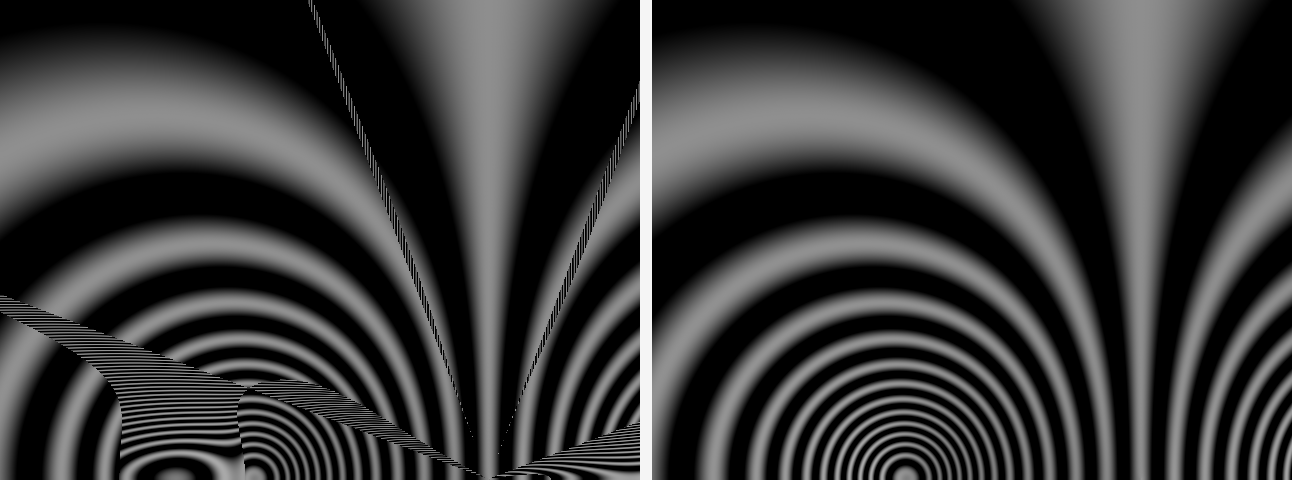
\includegraphics[width=\linewidth]{quilt-pair.png}
  \caption{\figlead{The handover quilt, and its cure.} Two concentric
  families of identical pitch and centre, one carrying a steep dipole field,
  at 1.87 pixels per member. Left: the envelope when the sum-or-difference
  choice is made from a finite difference of the fractional index over one
  pixel with the unit unwrap — an observer with a two-pixel window, which
  aliases below two pixels per member and hands the sum character pockets it
  never earned (hatched wedges, combs, dotted rays: the sum schedule holding
  carrier-pitch rims). Right: the same envelope with the choice made from the
  closed-form gradient. Both halves are the CPU mirror of the shipped
  compositing; the left is generated by the estimator, not by a resurrected
  shader. Script \texttt{quilt-figs.mjs}.}
  \label{fig:quilt}
\end{figure}

\section{Law III: integrability, the topology of the count}
\label{sec:integrability}

\begin{theorem}[Trichotomy]
\label{thm:trichotomy}
Let $F(p,\nu)=0$ be the incidence of a family (the point $p$ lies on the member
of continuous index $\nu$). The count $\nu(p)$ exists in exactly three ways:
as a global lift (the exact rung), as a lift on a cover with monodromy
$\pi_1\to\Z$ (the winding rung, whose defects carry quantized charge), or only
as a correspondence branched along the discriminant $\partial_\nu F=0$ (the
fold rung). A field moves $\Phi$ within its homotopy class or changes its
monodromy by a quantized amount, and never creates a discriminant.
\end{theorem}

\begin{proposition}[Carrier classification]
\label{prop:carriers}
Every closed-form family is the orbit of a seed curve under one of the four
one-parameter similarity flows of the plane (translation, rotation, dilation,
loxodrome) or a propagating front. An orbit family folds only where the flow
is tangent to the seed, so transverse seeds never fold; it winds exactly when
the flow has a rotational part. The alphabet is closed: the two carriers the
classification names that no catalogue shipped are the dilation clock
(geometric rings) and the loxodromic clock (the log spiral).
\end{proposition}

\begin{lemma}[Fold law]
\label{lem:foldlaw}
For a front whose member $n$ has support function $H_n$, gauge radius
$\rad_n$, and centre $c(n)$, the boundary-of-member map
$(u,n)\mapsto H_n(u)\,\hat u+H_n'(u)\,\hat u^{\perp}$ has Jacobian determinant
$-(H_n+H_n'')\,\partial_n H_n$ with $H_n+H_n''\ge0$ for a convex member. The
family folds exactly where the normal speed vanishes:
\[
  s\,H(w)\;-\;\rad_n\,\theta\,H'(w)\;+\;\langle c'(n),\hat u\rangle\;=\;0,
  \qquad w=u-n\theta .
\]
\end{lemma}

\begin{corollary}[Rotation folds everything but circles]
\label{cor:rotation}
With $\delta=0$ and $\theta\ne0$ the family folds at gauge radius
$\rad^\star=s/(\theta L)$, $L=\sup_w|H'(w)/H(w)|$, and nowhere before. For the
regular $k$-gon $L=\tan(\pi/k)$ and the first crossings appear at the vertices,
at Euclidean radius $R^\star=s/(\theta\sin(\pi/k))$; for an ellipse with
semi-axes $a\ge b$, $L=(a^2-b^2)/2ab$. For the circle $L=0$. Onsets measured
by brute nesting tests are within \foldWorstOnsetPct\% of these radii.
\end{corollary}

\begin{corollary}[The Mach condition]
\label{cor:mach}
With $\theta=0$ the family folds if and only if $\rad(-\delta)>s$: the drift
constant $m=\rad(-\delta)$ is a Mach number. Subsonic families nest forever,
supersonic ones fold from their first member along straight wake lines, and the
marginal drift $m=s$ is the sonic boundary.
\end{corollary}

\begin{proposition}[The reach of closed forms]
\label{prop:reach}
With $\theta=0$ the residual $h_p(\nu)$ is convex in $\nu$ for every gauge, so
translation is one closed form per gauge. If $\theta=2\pi a/b$ in lowest terms
the family splits into $b$ translated subfamilies, each convex, so the inverse
is $b$ closed forms (exact against brute force at $\theta=4\pi/7$). That is the
only mechanism a formula has: for any $\theta\ne0$ the interpolated incidence
$\{(p,\nu):h_p(\nu)=0\}$ is not semialgebraic, since a semialgebraic incidence
would force $\nu\mapsto\nu\lVert\delta\rVert\cos(\nu\theta+\beta)$ to be
algebraic over $\R(\nu)$. Beyond it the count is multivalued, with branches
through a point growing linearly in radius (\foldBranchCounts).
\end{proposition}

\begin{figure}[t]
  \centering
  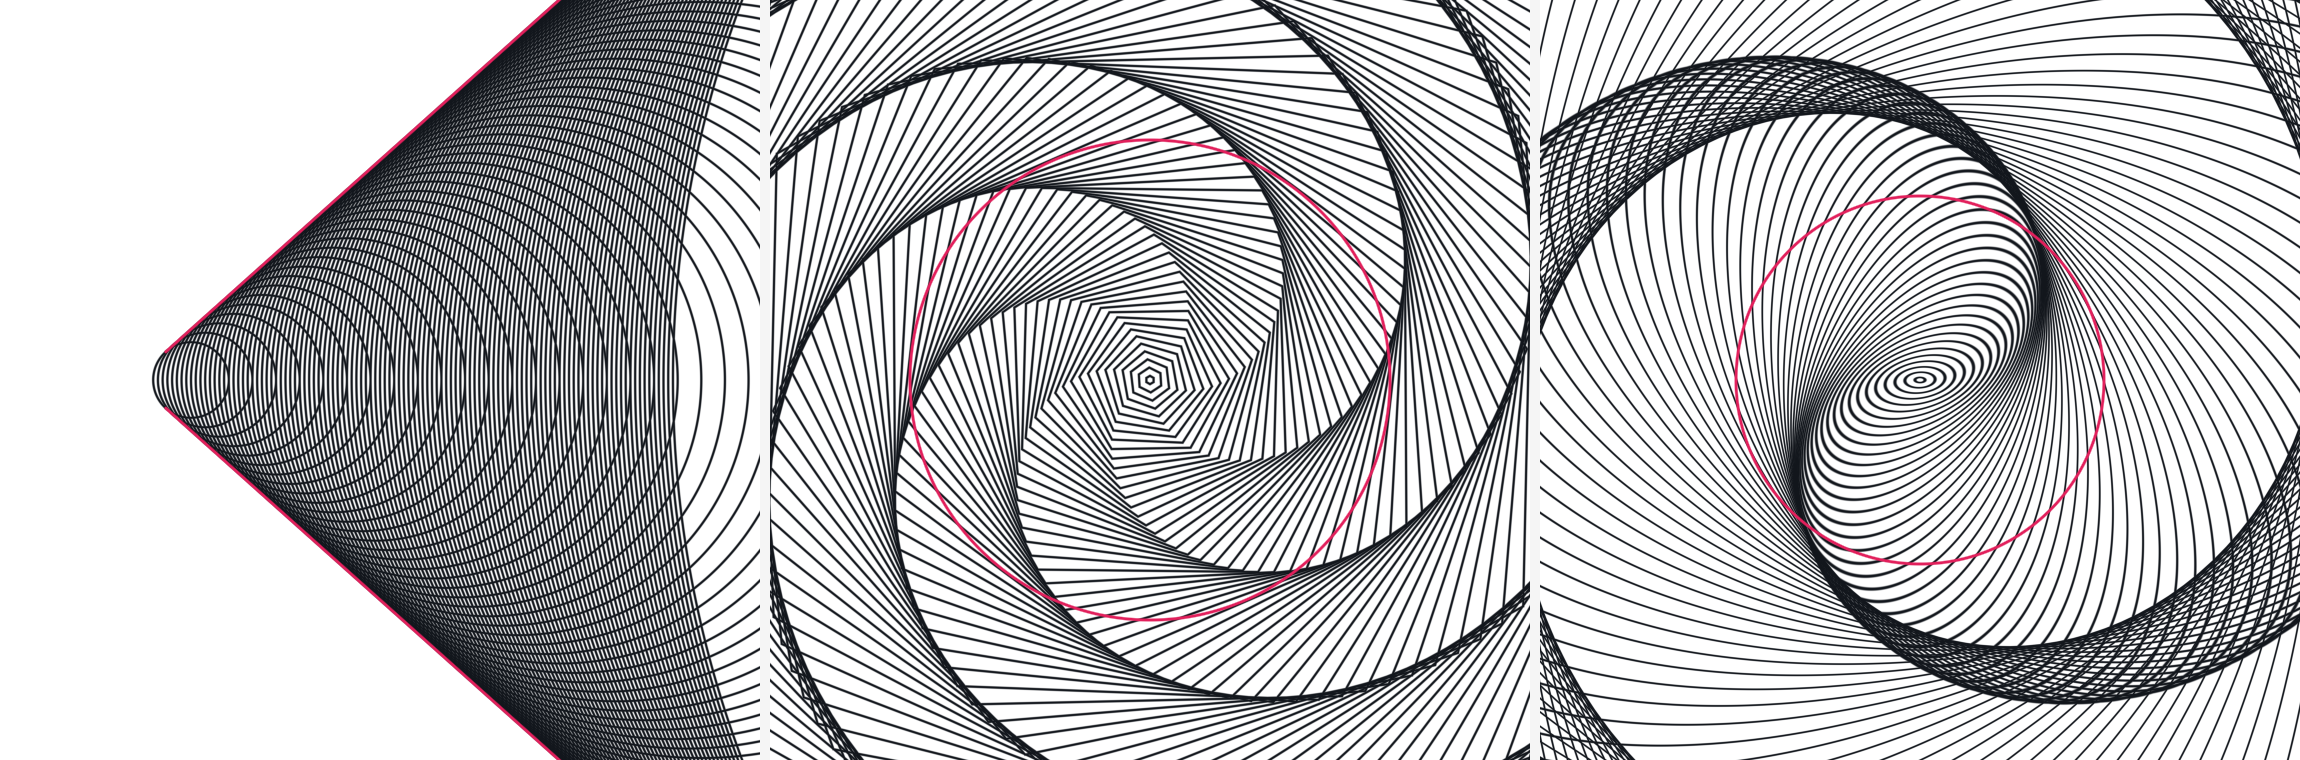
\includegraphics[width=\linewidth]{fold-law.png}
  \caption{\figlead{The fold law drawn.} Predicted caustics (crimson) over
  brute-force renders that never saw the support calculus; the onset radius
  dashed. Imported from the companion draft's \texttt{foldlaw-figs.mjs}.}
  \label{fig:foldlaw}
\end{figure}

\begin{proposition}[Defects]
\label{prop:defects}
A circle-valued field of integer amount $A$ composed into a layer's index
changes the monodromy of $\Phi$: each zero of winding number $q$ ends $Aq$
fringes, the signed count of fringe endings inside any loop is $A$ times the
enclosed charge, and the fringe law fails inside the core $r^\star=2As/\pi$
where $\het$ crosses $\tfrac14$. Measured on \defProbes\ probes with charges up
to \defChargeMax, exact; the core law within $\defCoreWorst$.
\end{proposition}

\placeholder{the fork grating}{Provisional assets \texttt{defect-fork.png},
\texttt{defect-pair.png}, \texttt{defect-envelope.png}: one column, compressed
from the companion's \S5. (P3.)}

\section{Predictions, measured}
\label{sec:predictions}

Every claim above with a number behind it, its measured value, the gate the
experiment must pass for this document to build, and the script that owns it.
The table is generated by \texttt{tools/numbers.mjs} from the scripts' own
data files; a failing gate stops the build.

\begin{table}[h]
  \centering\small
  % GENERATED by paper/tools/numbers.mjs -- do not edit by hand.
\begin{tabular}{@{}p{0.37\linewidth}p{0.26\linewidth}p{0.13\linewidth}l@{}}
\toprule
Claim & Measured & Gate & Script \\
\midrule
Duty null: the $2{:}1$ station at coarse duty $1/2$ & $6{,}305\times$ below its neighbours & $>10\times$ & \texttt{dutynull.mjs} \\
Duty nulls: the $3{:}1$ station at $1/3$ and $2/3$ & $3{,}458\times$, $2{,}549\times$ & $>10\times$ each & \texttt{dutynull.mjs} \\
Temporal selection: rates $(1,2)$ keep the station, $(1,1)$ and $(2,1)$ wash it & $14{,}668\times$; kept to 0.09\% of the still & $>30\times$; $<2\%$ & \texttt{exposure.mjs} \\
Exact sweep: Gauss-3 chain against a 65\,536-tap truth & $7\times 10^{-5}$ over 480 scenes & $<2\times10^{-3}$ & \texttt{exactsweep.mjs} \\
Exact sweep: every corner named (Gauss-4) & $2\times 10^{-8}$ & $<10^{-5}$ & \texttt{exactsweep.mjs} \\
Exact sweep: the shipped shader against its double-precision twin & $3\times 10^{-7}$ & $<10^{-4}$ & \texttt{exactsweep.mjs} \\
Observer: a window is the torus multiplier & $9\times 10^{-8}$ & $<5\times10^{-5}$ & \texttt{observer.mjs} \\
Observer: the curvature remainder is the multiplier's second derivative & residual $3\times 10^{-2}$ of the remainder & $<0.1$ & \texttt{observer.mjs} \\
Observer: additive light has no linear beat & $8\times 10^{-17}$ & $<10^{-10}$ & \texttt{observer.mjs} \\
Observer: a squaring front end mints it at $\hat g_1(1)\hat g_2(1)/2$ & 0.0403 vs 0.0403 & rel.\ $<10^{-6}$ & \texttt{observer.mjs} \\
Observer: hard ink is observer-proof & $2\times 10^{-17}$ & $<10^{-12}$ & \texttt{observer.mjs} \\
Observer: soft ink reopens the null under squaring, linearly in the ramp & $3\times 10^{-3}$, $7\times 10^{-3}$, $10^{-2}$ & monotone, $>10^{-4}$ & \texttt{observer.mjs} \\
Fold law: onset radii of rotating gauges and Mach drifts & within 2.8\% & every onset gate & \texttt{foldlaw.mjs} \\
Fold law: crossings are born on the caustic & within 0.07 world units & every birth gate & \texttt{foldlaw.mjs} \\
Untwist: rational twists split into convex classes & exact at $\theta=4\pi/7$ & splits exact & \texttt{foldlaw.mjs} \\
Branch counts grow linearly in radius & 3, 5, 9, 21, 41 & as predicted & \texttt{foldlaw.mjs} \\
Defects: fringe endings count the enclosed charge & 22 probes exact, charges to 10 & exact & \texttt{defects.mjs} \\
Defects: the core radius $2As/\pi$ & within $10^{-4}$ & gated & \texttt{defects.mjs} \\
Selection: record beats are convergents & 207 of 207 & no mismatch & \texttt{convergents.mjs} \\
Selection: the reduction window names the brute-force winner & 99.8\% of 4{,}000 & misses 1 & \texttt{convergents.mjs} \\
\bottomrule
\end{tabular}

  \caption{\figlead{The gated predictions.} No claim without a number; no
  number without a script.}
  \label{tab:predictions}
\end{table}

\section{Coda: the instrument}
\label{sec:coda}

% P4: one paragraph. The tool exists (WebGPU, closed-form solvers, the exact
% sweep), the zoo method (golden-image regression through the real GPU), and
% the companion paper for every engineering claim. The plate and teaser assets
% appear as running examples above, not as a gallery.

% Discussion, one honest paragraph: the resonance web. Stations are closed
% orbits, deserts are badly approximable directions, the visible drawing lives
% at their boundary graded by the amplitude weight. Applications in one
% sentence. No cosmology.


\end{document}
